\documentclass[11pt,a4paper,french,twoside]{PMCours}
\usepackage{hyperref}

\newcounter{activite}
\newcommand{\activite}{\subsubsection*{Activité~\refstepcounter{activite}\theactivite}}

\begin{document}
\TitreISN{Classe de Terminale}{Année 2021--2022}
{Numérique et Sciences Informatiques}{TP/TD 4 : Arbres, Arbres Binaires de Recherche et Parcours}
\section*{Problème : Arbres}
\subsection*{Partie 1 : Généralités}
On définit de manière classique en langage Python la classe suivante, permettant de définir les noeuds des arbres binaires. 
\begin{Python}
class Noeud : 
	def __init__(self,g,v,d):
		self.gauche = g
		self.valeur = v
		self.droit = d
\end{Python}
dans lequel :
\begin{itemize}
\item \code{v}, suivant les exemples, contient une chaine de caractères, un type numérique, etc...
\item \code{g} et \code{d} sont des instances de la classe \code{Noeud}, représentant respectivement les racines des sous-arbres gauche et droit du noeud créé, valant éventuellement \code{None} si les sous-arbres sont vides. 
\end{itemize}
\begin{enumerate}
\item \begin{enumerate}
\item Représenter l'arbre obtenu en suivant les instructions suivantes.
\begin{Python}
noeudD=Noeud(None,'D',None)
noeudE=Noeud(None,'E',None)
noeudF=Noeud(None,'F',None)
noeudA=Noeud(noeudE,'A',noeudF)
noeudC=Noeud(noeudD,'C',noeudA)
\end{Python}
\item Donner les résultats des appels suivants :
\begin{itemize}
\item \code{noeudC.gauche.valeur}
\item \code{noeudC.gauche.droit}
\item \code{noeudA.gauche.droit}
\end{itemize}
\end{enumerate}
\item \begin{enumerate}
\item Donner un jeu d'instructions permettant de créer l'arbre représenté ci-dessous. (On pourra au besoin appeler \code{noeud1} le noeud dont la valeur est \code{1}, etc...)
\begin{center}
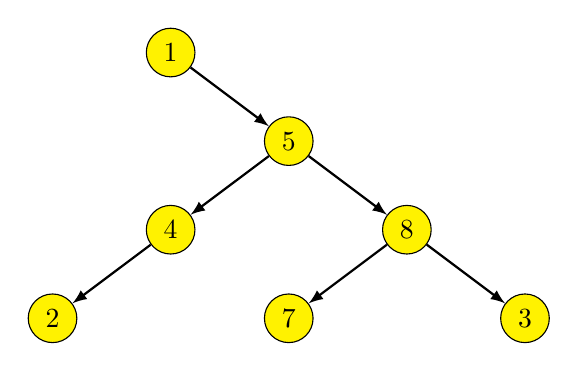
\begin{tikzpicture}[xscale=.5,yscale=.5]
% Styles (MODIFIABLES)
\tikzstyle{fleche}=[->,>=latex,thick]
\tikzstyle{noeud}=[fill=yellow,circle,draw]
\tikzstyle{feuille}=[fill=orange,circle,draw]
% Dimensions (MODIFIABLES)
\def\DistanceInterNiveaux{3}
\def\DistanceInterFeuilles{2}
% Dimensions calculées (NON MODIFIABLES)
\def\NiveauA{(-0)*\DistanceInterNiveaux}
\def\NiveauB{(-.75)*\DistanceInterNiveaux}
\def\NiveauC{(-1.5)*\DistanceInterNiveaux}
\def\NiveauD{(-2.25)*\DistanceInterNiveaux}
\def\InterFeuilles{(.75)*\DistanceInterFeuilles}
% Noeuds (MODIFIABLES : Styles et Coefficients d'InterFeuilles)
\node[noeud] (R) at ({(-2)*\InterFeuilles},{\NiveauA}) {$1$};
\node[noeud] (Ra) at ({(0)*\InterFeuilles},{\NiveauB}) {$5$};
\node[noeud] (Raa) at ({(-2)*\InterFeuilles},{\NiveauC}) {$4$};
\node[noeud] (Rab) at ({(2)*\InterFeuilles},{\NiveauC}) {$8$};
\node[noeud] (Raaa) at ({(-4)*\InterFeuilles},{\NiveauD}) {$2$};
\node[noeud] (Raba) at ({(0)*\InterFeuilles},{\NiveauD}) {$7$};
\node[noeud] (Rabb) at ({(4)*\InterFeuilles},{\NiveauD}) {$3$};
% Arcs (MODIFIABLES : Styles)
\draw[fleche] (R)--(Ra);
\draw[fleche] (Ra)--(Raa);
\draw[fleche] (Ra)--(Rab);
\draw[fleche] (Raa)--(Raaa);
\draw[fleche] (Rab)--(Raba);
\draw[fleche] (Rab)--(Rabb);
\end{tikzpicture}\\
\title{Arbre 2}
\end{center}
\item Rappeler la définition de la taille et de la hauteur d'un arbre binaire, donner leurs valeurs pour l'Arbre 2.
\end{enumerate}
\item On se donne la fonction 
\begin{Python}
def f(noeud):
	if noeud is None :
		return 0
	else :
		return noeud.valeur+f(noeud.gauche)+f(noeud.droit)
\end{Python} 
\begin{enumerate}
\item Que renvoie \code{f} quand on l'applique à une feuille d'un arbre ? 
\item Appliquer \code{f} au noeud-racine de l'Arbre 2, en décrivant brièvement son déroulement.\\ Quelle valeur la fonction renvoie-t-elle ? 
\item Décrire sans paraphraser ce que fait la fonction.
\end{enumerate} 
\end{enumerate}
\subsection*{Partie 2 : Arbres Binaires de Recherche}
\begin{Definition}{Arbre Binaire de Recherche (ABR)}
Un arbre binaire de recherche (ABR) est un un arbre binaire vérifiant la propriété suivante.
Pour tout noeud \code{n} de l'arbre (et de manière récursive), 
\begin{itemize}
\item tout noeud situé sur l'arbre gauche de \code{n} a une valeur 
strictement inférieure à la valeur de \code{n}
\item tout noeud situé sur l'arbre droit de \code{n} a une valeur strictement supérieure à la valeur de \code{n}
\end{itemize}
\end{Definition}\ \\
Ainsi, l'Arbre 3 ci dessous est un ABR tandis que l'Arbre 4 n'en est pas un. 
\begin{multicols}{2}
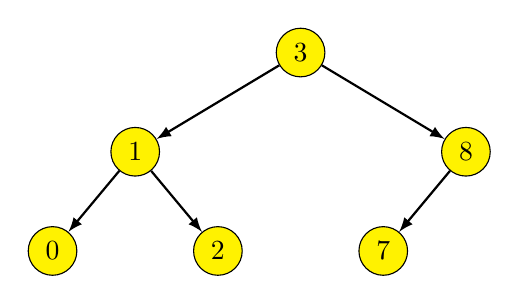
\begin{tikzpicture}[xscale=.7,yscale=.7]
% Styles (MODIFIABLES)
\tikzstyle{fleche}=[->,>=latex,thick]
\tikzstyle{noeud}=[fill=yellow,circle,draw]
\tikzstyle{feuille}=[fill=orange,circle,draw]
% Dimensions (MODIFIABLES)
\def\DistanceInterNiveaux{3}
\def\DistanceInterFeuilles{2}
% Dimensions calculées (NON MODIFIABLES)
\def\NiveauA{(-0)*\DistanceInterNiveaux}
\def\NiveauB{(-.6)*\DistanceInterNiveaux}
\def\NiveauC{(-1.2)*\DistanceInterNiveaux}
\def\NiveauD{(-1.8)*\DistanceInterNiveaux}
\def\InterFeuilles{(.75)*\DistanceInterFeuilles}
% Noeuds (MODIFIABLES : Styles et Coefficients d'InterFeuilles)
\node[noeud] (R) at ({(0)*\InterFeuilles},{\NiveauA}) {$3$};
\node[noeud] (Ra) at ({(-2)*\InterFeuilles},{\NiveauB}) {$1$};
\node[noeud] (Rb) at ({(2)*\InterFeuilles},{\NiveauB}) {$8$};
\node[noeud] (Raa) at ({(-3)*\InterFeuilles},{\NiveauC}) {$0$};
\node[noeud] (Rab) at ({(-1)*\InterFeuilles},{\NiveauC}) {$2$};
\node[noeud] (Rba) at ({(1)*\InterFeuilles},{\NiveauC}) {$7$};
% Arcs (MODIFIABLES : Styles)
\draw[fleche] (R)--(Ra);
\draw[fleche] (R)--(Rb);
\draw[fleche] (Ra)--(Raa);
\draw[fleche] (Ra)--(Rab);
\draw[fleche] (Rb)--(Rba);
\end{tikzpicture}\medskip \\
. \hskip 2cm \title{Arbre 3}

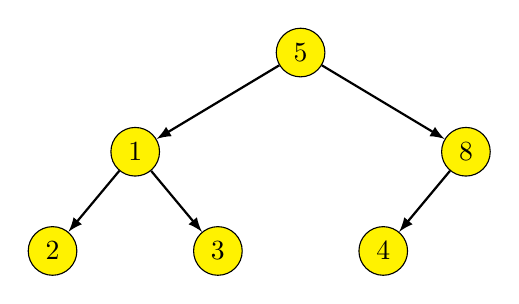
\begin{tikzpicture}[xscale=.7,yscale=.7]
% Styles (MODIFIABLES)
\tikzstyle{fleche}=[->,>=latex,thick]
\tikzstyle{noeud}=[fill=yellow,circle,draw]
\tikzstyle{feuille}=[fill=orange,circle,draw]
% Dimensions (MODIFIABLES)
\def\DistanceInterNiveaux{3}
\def\DistanceInterFeuilles{2}
% Dimensions calculées (NON MODIFIABLES)
\def\NiveauA{(-0)*\DistanceInterNiveaux}
\def\NiveauB{(-.6)*\DistanceInterNiveaux}
\def\NiveauC{(-1.2)*\DistanceInterNiveaux}
\def\NiveauD{(-1.8)*\DistanceInterNiveaux}
\def\InterFeuilles{(.75)*\DistanceInterFeuilles}
% Noeuds (MODIFIABLES : Styles et Coefficients d'InterFeuilles)
\node[noeud] (R) at ({(0)*\InterFeuilles},{\NiveauA}) {$5$};
\node[noeud] (Ra) at ({(-2)*\InterFeuilles},{\NiveauB}) {$1$};
\node[noeud] (Rb) at ({(2)*\InterFeuilles},{\NiveauB}) {$8$};
\node[noeud] (Raa) at ({(-3)*\InterFeuilles},{\NiveauC}) {$2$};
\node[noeud] (Rab) at ({(-1)*\InterFeuilles},{\NiveauC}) {$3$};
\node[noeud] (Rba) at ({(1)*\InterFeuilles},{\NiveauC}) {$4$};
% Arcs (MODIFIABLES : Styles)
\draw[fleche] (R)--(Ra);
\draw[fleche] (R)--(Rb);
\draw[fleche] (Ra)--(Raa);
\draw[fleche] (Ra)--(Rab);
\draw[fleche] (Rb)--(Rba);
\end{tikzpicture}\medskip \\
. \hskip 2cm \title{Arbre 4}

\end{multicols}
En effet, pour l'Arbre 4,
\begin{itemize}
\item \code{noeud2} est sur l'arbre gauche de \code{noeud1} mais $2>1$
\item \code{noeud4} est sur l'arbre droit de \code{noeud5} mais $4<5$
\end{itemize}
\begin{enumerate}
\item
\begin{enumerate}
\item Déterminer un ABR de hauteur 2 constitué de trois noeuds de valeurs respectives \code{1} , \code{2}, \code{3}
\item Déterminer un ABR de hauteur 3 constitué de six noeuds de valeurs respectives \code{1} ,... ,\code{6}.
\end{enumerate}
\item Réaliser le parcours infixe de l'arbre 3. Qu'observe-t-on ? Justifier brièvement.
\item \begin{enumerate}
\item On se donne l'ABR suivant ne contenant que des valeurs entières.\\
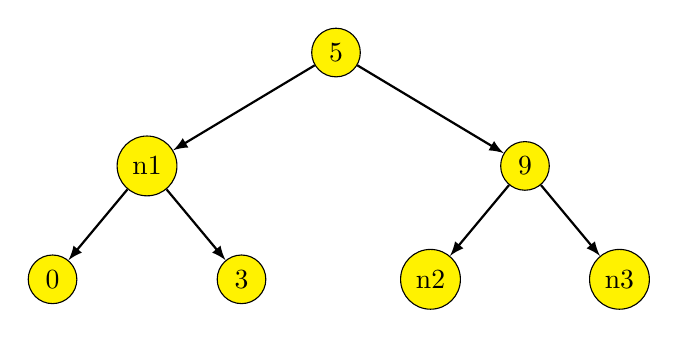
\begin{tikzpicture}[xscale=.8,yscale=.8]
% Styles (MODIFIABLES)
\tikzstyle{fleche}=[->,>=latex,thick]
\tikzstyle{noeud}=[fill=yellow,circle,draw]
\tikzstyle{feuille}=[fill=orange,circle,draw]
% Dimensions (MODIFIABLES)
\def\DistanceInterNiveaux{3}
\def\DistanceInterFeuilles{2}
% Dimensions calculées (NON MODIFIABLES)
\def\NiveauA{(-0)*\DistanceInterNiveaux}
\def\NiveauB{(-.6)*\DistanceInterNiveaux}
\def\NiveauC{(-1.2)*\DistanceInterNiveaux}
\def\NiveauD{(-1.8)*\DistanceInterNiveaux}
\def\InterFeuilles{(.75)*\DistanceInterFeuilles}
% Noeuds (MODIFIABLES : Styles et Coefficients d'InterFeuilles)
\node[noeud] (R) at ({(0)*\InterFeuilles},{\NiveauA}) {$5$};
\node[noeud] (Ra) at ({(-2)*\InterFeuilles},{\NiveauB}) {\code{n1}};
\node[noeud] (Rb) at ({(2)*\InterFeuilles},{\NiveauB}) {$9$};
\node[noeud] (Raa) at ({(-3)*\InterFeuilles},{\NiveauC}) {$0$};
\node[noeud] (Rab) at ({(-1)*\InterFeuilles},{\NiveauC}) {$3$};
\node[noeud] (Rba) at ({(1)*\InterFeuilles},{\NiveauC}) {\code{n2}};
\node[noeud] (Rbb) at ({(3)*\InterFeuilles},{\NiveauC}) {\code{n3}};
% Arcs (MODIFIABLES : Styles)
\draw[fleche] (R)--(Ra);
\draw[fleche] (R)--(Rb);
\draw[fleche] (Ra)--(Raa);
\draw[fleche] (Ra)--(Rab);
\draw[fleche] (Rb)--(Rba);
\draw[fleche] (Rb)--(Rbb);
\end{tikzpicture}
\begin{enumerate}
\item La valeur 4 peut-elle être présente dans l'arbre ? Si oui, à quel noeud ?
\item La valeur 7 peut-elle être présente dans l'arbre ? Si oui, à quel noeud ?
\item Plus généralement, en justifiant brièvement, quelles valeurs peuvent avoir les noeuds \code{n1}, \code{n2} et \code{n3} ?
\end{enumerate}
\item En vous aidant des raisonnements développés à la question précédente, compléter le code suivant pour en faire le code d'une fonction s'appelant \code{rechercheABR} prenant comme argument un noeud-racine d'un ABR \code{n} et un nombre \code{elt} et renvoyant \code{True} si \code{elt} est un élément de l'arbre et \code{False} sinon. 
\begin{Python}
def #à compléter1
	a=n
	while a is not None :
		if a.valeur == elt :
			return #à compléter2
		elif #à compléter3
			a=a.gauche
		else : 
			#à compléter4
	return False
\end{Python}
\end{enumerate}
\item \begin{enumerate}
\item On veut construire un ABR dont les noeuds auront comme valeur les éléments (supposés tous différents) d'une liste donnée.\\
Le premier élément de la liste constituera la racine de l'arbre, le second sera placé sur l'arbre gauche ou l'arbre droit suivant sa valeur, etc... \\
Par exemple, avec \code{L=[0,10,7,-5,8,11,3,-2]}, les premières étapes sont : 
\begin{multicols}{4}
 
.\hskip -2cm 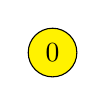
\begin{tikzpicture}[xscale=.7,yscale=.7]
% Styles (MODIFIABLES)
\tikzstyle{fleche}=[->,>=latex,thick]
\tikzstyle{noeud}=[fill=yellow,circle,draw]
\tikzstyle{feuille}=[fill=orange,circle,draw]
% Dimensions (MODIFIABLES)
\def\DistanceInterNiveaux{3}
\def\DistanceInterFeuilles{2}
% Dimensions calculées (NON MODIFIABLES)
\def\NiveauA{(-0)*\DistanceInterNiveaux}
\def\NiveauB{(-.6)*\DistanceInterNiveaux}
\def\NiveauC{(-1.2)*\DistanceInterNiveaux}
\def\NiveauD{(-1.8)*\DistanceInterNiveaux}
\def\InterFeuilles{(.75)*\DistanceInterFeuilles}
% Noeuds (MODIFIABLES : Styles et Coefficients d'InterFeuilles)
\node[noeud] (R) at ({(0)*\InterFeuilles},{\NiveauA}) {$0$};
% Arcs (MODIFIABLES : Styles)
\end{tikzpicture} 
\ \\ \\ \\ \\   
.\hskip -2cm 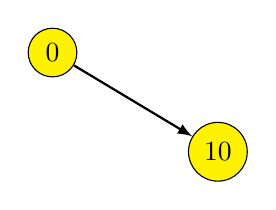
\begin{tikzpicture}[xscale=.7,yscale=.7]
% Styles (MODIFIABLES)
\tikzstyle{fleche}=[->,>=latex,thick]
\tikzstyle{noeud}=[fill=yellow,circle,draw]
\tikzstyle{feuille}=[fill=orange,circle,draw]
% Dimensions (MODIFIABLES)
\def\DistanceInterNiveaux{3}
\def\DistanceInterFeuilles{2}
% Dimensions calculées (NON MODIFIABLES)
\def\NiveauA{(-0)*\DistanceInterNiveaux}
\def\NiveauB{(-.6)*\DistanceInterNiveaux}
\def\NiveauC{(-1.2)*\DistanceInterNiveaux}
\def\NiveauD{(-1.8)*\DistanceInterNiveaux}
\def\InterFeuilles{(.75)*\DistanceInterFeuilles}
% Noeuds (MODIFIABLES : Styles et Coefficients d'InterFeuilles)
\node[noeud] (R) at ({(0)*\InterFeuilles},{\NiveauA}) {$0$};
\node[noeud] (Rb) at ({(2)*\InterFeuilles},{\NiveauB}) {$10$};
% Arcs (MODIFIABLES : Styles)
\draw[fleche] (R)--(Rb);
\end{tikzpicture}    
     
      
.\hskip -2cm 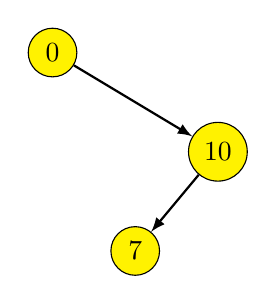
\begin{tikzpicture}[xscale=.7,yscale=.7]
% Styles (MODIFIABLES)
\tikzstyle{fleche}=[->,>=latex,thick]
\tikzstyle{noeud}=[fill=yellow,circle,draw]
\tikzstyle{feuille}=[fill=orange,circle,draw]
% Dimensions (MODIFIABLES)
\def\DistanceInterNiveaux{3}
\def\DistanceInterFeuilles{2}
% Dimensions calculées (NON MODIFIABLES)
\def\NiveauA{(-0)*\DistanceInterNiveaux}
\def\NiveauB{(-.6)*\DistanceInterNiveaux}
\def\NiveauC{(-1.2)*\DistanceInterNiveaux}
\def\NiveauD{(-1.8)*\DistanceInterNiveaux}
\def\InterFeuilles{(.75)*\DistanceInterFeuilles}
% Noeuds (MODIFIABLES : Styles et Coefficients d'InterFeuilles)
\node[noeud] (R) at ({(0)*\InterFeuilles},{\NiveauA}) {$0$};
\node[noeud] (Rb) at ({(2)*\InterFeuilles},{\NiveauB}) {$10$};
\node[noeud] (Rba) at ({(1)*\InterFeuilles},{\NiveauC}) {$7$};
% Arcs (MODIFIABLES : Styles)
\draw[fleche] (R)--(Rb);
\draw[fleche] (Rb)--(Rba);
\end{tikzpicture}           
        
.\hskip -2cm 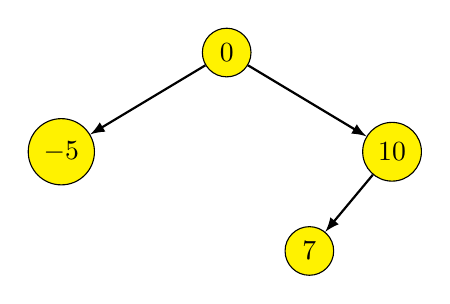
\begin{tikzpicture}[xscale=.7,yscale=.7]
% Styles (MODIFIABLES)
\tikzstyle{fleche}=[->,>=latex,thick]
\tikzstyle{noeud}=[fill=yellow,circle,draw]
\tikzstyle{feuille}=[fill=orange,circle,draw]
% Dimensions (MODIFIABLES)
\def\DistanceInterNiveaux{3}
\def\DistanceInterFeuilles{2}
% Dimensions calculées (NON MODIFIABLES)
\def\NiveauA{(-0)*\DistanceInterNiveaux}
\def\NiveauB{(-.6)*\DistanceInterNiveaux}
\def\NiveauC{(-1.2)*\DistanceInterNiveaux}
\def\NiveauD{(-1.8)*\DistanceInterNiveaux}
\def\InterFeuilles{(.75)*\DistanceInterFeuilles}
% Noeuds (MODIFIABLES : Styles et Coefficients d'InterFeuilles)
\node[noeud] (R) at ({(0)*\InterFeuilles},{\NiveauA}) {$0$};
\node[noeud] (Rb) at ({(2)*\InterFeuilles},{\NiveauB}) {$10$};
\node[noeud] (Ra) at ({(-2)*\InterFeuilles},{\NiveauB}) {$-5$};
\node[noeud] (Rba) at ({(1)*\InterFeuilles},{\NiveauC}) {$7$};
% Arcs (MODIFIABLES : Styles)
\draw[fleche] (R)--(Ra);
\draw[fleche] (R)--(Rb);
\draw[fleche] (Rb)--(Rba);
\end{tikzpicture}          
\end{multicols}
Donner l'ABR complet obtenu en ajoutant les noeuds correspondant au reste de la liste.  
\item En vous aidant des raisonnements développés à la question précédente et du code de la fonction \code{rechercheABR}, donner le code d'une fonction s'appelant \code{construireABR} prenant comme argument une liste d'entiers deux à deux différents \code{L} et renvoyant la racine d'un ABR construit à partir des éléments de la liste. \medskip\\ 
On pourra s'aider du canevas suivant : 
\begin{itemize}
\item création de la racine \code{rac}
\item pour chaque autre élément \code{L[i]} de la liste \code{L},
\begin{itemize}
\item on se place à la racine avec \code{a=rac}
\item tant que \code{a} n'est pas \code{None}
\begin{itemize}
\item on stocke l'ancien \code{a} dans une variable \code{b} et on remplace \code{a} par \code{a.gauche} ou \code{a.droit} suivant le résultat du test \code{L[i]}\code{>} \code{valeur} de \code{a}.
\end{itemize}
\item on crée alors un nouveau noeud, de valeur \code{L[i]}, et on le place à gauche ou à droite de \code{b} en suivant la règle des ABR .
\end{itemize}
\end{itemize}
\end{enumerate}
\end{enumerate}
\subsection*{Partie 3 : Parcours d'arbre en largeur}
\begin{Definition}{Parcours en largeur d'un arbre}
Un parcours en largeur d'un arbre est un parcours dans lequel tous les noeuds à même distance de la racine sont listés consécutivement.
\end{Definition}\ \\
Par exemple, \medskip\\
\begin{tabular}{p{8cm}p{8cm}}
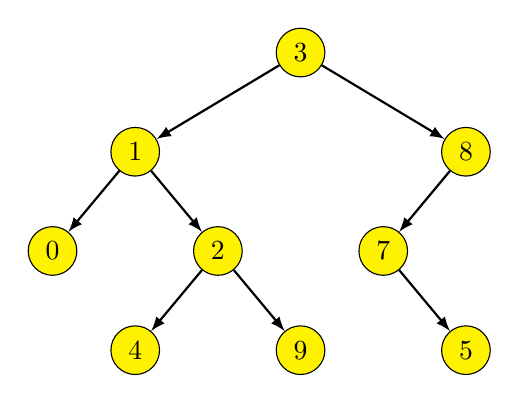
\begin{tikzpicture}[xscale=.7,yscale=.7]
% Styles (MODIFIABLES)
\tikzstyle{fleche}=[->,>=latex,thick]
\tikzstyle{noeud}=[fill=yellow,circle,draw]
\tikzstyle{feuille}=[fill=orange,circle,draw]
% Dimensions (MODIFIABLES)
\def\DistanceInterNiveaux{3}
\def\DistanceInterFeuilles{2}
% Dimensions calculées (NON MODIFIABLES)
\def\NiveauA{(-0)*\DistanceInterNiveaux}
\def\NiveauB{(-.6)*\DistanceInterNiveaux}
\def\NiveauC{(-1.2)*\DistanceInterNiveaux}
\def\NiveauD{(-1.8)*\DistanceInterNiveaux}
\def\InterFeuilles{(.75)*\DistanceInterFeuilles}
% Noeuds (MODIFIABLES : Styles et Coefficients d'InterFeuilles)
\node[noeud] (R) at ({(0)*\InterFeuilles},{\NiveauA}) {$3$};
\node[noeud] (Ra) at ({(-2)*\InterFeuilles},{\NiveauB}) {$1$};
\node[noeud] (Rb) at ({(2)*\InterFeuilles},{\NiveauB}) {$8$};
\node[noeud] (Raa) at ({(-3)*\InterFeuilles},{\NiveauC}) {$0$};
\node[noeud] (Rab) at ({(-1)*\InterFeuilles},{\NiveauC}) {$2$};
\node[noeud] (Rba) at ({(1)*\InterFeuilles},{\NiveauC}) {$7$};
\node[noeud] (Raba) at ({(-2)*\InterFeuilles},{\NiveauD}) {$4$};
\node[noeud] (Rabb) at ({(0)*\InterFeuilles},{\NiveauD}) {$9$};
\node[noeud] (Rbab) at ({(2)*\InterFeuilles},{\NiveauD}) {$5$};

% Arcs (MODIFIABLES : Styles)
\draw[fleche] (R)--(Ra);
\draw[fleche] (R)--(Rb);
\draw[fleche] (Ra)--(Raa);
\draw[fleche] (Ra)--(Rab);
\draw[fleche] (Rb)--(Rba);
\draw[fleche] (Rab)--(Raba);
\draw[fleche] (Rab)--(Rabb);
\draw[fleche] (Rba)--(Rbab);
\end{tikzpicture}
& \begin{tabular}{p{8cm}}
Un parcours en largeur de l'arbre ci-contre est : \\
\code{3 - 1 - 8  - 0 - 2 - 7 - 4 - 9 - 5} \ \\ \\ \\ \\ \\ \\ \\ \\ 
\end{tabular}
\end{tabular}\medskip\\
.\vskip -1.5cm La programmation d'un tel parcours nécessite l'utilisation d'une file.\\
On suppose que l'on dispose d'une classe \code{File} possédant une interface contenant les fonctions usuelles, permettant de créer une file vide, de tester si une file est vide, et d'enfiler/de défiler un élément. \medskip\\
Dès lors, on peut décrire l'algorithme comme suit : 
\begin{Python}
Fonction parcours_largeur(n) 
	f est une file vide
	enfiler n dans f
	Tant que f est non vide 
		defiler f dans s.
		afficher s
		pour les enfants t de s : 
			enfiler t dans f
\end{Python}	
\begin{enumerate}
\item Observer le déroulement de l'algorithme \code{parcours\_largeur} appliqué à l'arbre 5. \\
On tiendra compte lors du déroulement du contenu de \code{f}, de \code{s} et des valeurs affichées.
\item Implémenter une classe \code{File} puis la fonction \code{parcours\_largeur} en langage Python.
\item Créer l'arbre 5.\\
On pourra compléter le code de la fonction suivante : 
\begin{Python}
def cree_arbre() :
    L=[]
    for k in #à compléter 1 :
        L.append(Noeud(None,k,None))
    for tu in #à compléter 2 :
        L[tu[0]].gauche=L[tu[1]]
    for tu in #à compléter 3 :
        L[tu[0]].droit=L[tu[1]]
    return L[3]
\end{Python}
et récupérer la racine de l'arbre 5 dans une variable \code{n3}.
\item Vérifier le bon fonctionnement de \code{parcours\_largeur} en la testant sur \code{n3}.
\item On suppose que l'on dispose d'une classe pile possédant une interface contenant les fonctions usuelles, permettant de créer une pile vide, de tester si une pile est vide, et d'empiler/de dépiler un élément. \medskip\\
Dès lors, on considère l'algorithme : 
\begin{Python}
Fonction parcours_mystere(n) 
	f est une pile vide
	empiler n dans f
	Tant que f est non vide 
		depiler f dans s.
		afficher s
		pour les enfants t de s : 
			empiler t dans f
\end{Python}	
\begin{enumerate}
\item Appliquer l'algorithme \code{parcours\_mystere} à l'arbre 5. Quel affichage obtient-on ? 
\item Comment appelle-t-on un tel parcours ?
\item Implémenter une classe Pile puis la fonction \code{parcours\_mystere} en langage Python.
\item Vérifier alors le bon fonctionnement de l\code{parcours\_mystere} en la testant sur \code{n3}.
\end{enumerate}
\end{enumerate}
\end{document}

